\section{Extensible Memory Layout Structures}\label{sec:layouts}

One of the most significant challenges of the outlined problem is to create an indexing abstraction that would follow the fundamental code design principles (especially in object-oriented programming, which is one of the most widely adopted paradigms), thus allowing the programmer to write neat and maintainable code, whilst minimizing performance overhead and making heavy use of the compile-time optimizations.

In this work, we propose using first-class indexing structures which can be detached entirely from the allocated memory and the data structures themselves. The indexing structure has a specific type (templated class) composed of predefined base types and a corresponding instance (object). This way, the information being passed to the layout-agnostic algorithm is divided into two parts:
\begin{itemize}
\item the data type passed via (inferred) template parameter, which bears the structure and constant parameters,
\item and the object, which bears all dynamic parameters (such as sizes of non-constant dimensions of the data structure).
\end{itemize}

Before we focus on the benefits, let us emphasize the C++ cornerstones of \Noarr{} that are pretty important for understanding the main principles (details are provided in Section~\ref{sec:implementation}).

\begin{itemize}
    \item The indexing structure type composition is straightforward as the user merely combines predefined \Noarr{} templated classes. Furthermore, thanks to the templating system, it is easy to create partially-defined structures, thus promoting code reusability. The construction of derived or augmented types (like binding the constant dimensions) is implemented in a functional manner, which is quite comprehensive and easy to write. Finally, modern C++ constructs like \mintinline{c++}{auto} or template type inference make these type modifications easier to handle since only the instance object is passed down.
    \item The dimensions of the data structure are denoted using chars (typically letters), which are much more mnemonic than numbers or the order of definition. Furthermore, they can be used to define additional abstraction so that structures with the same set of named dimensions can be treated as compatible, regardless of the order of their definition or their actual layout representation.
    \item Finally, the implementation makes heavy use of \mintinline{c++}{constexpr} functions which allow the compiler to be inlined, resolve, and even precompute many pieces of the layout-related code, thus making it more efficient. For instance, the constant dimensions can be translated into the expressions where the actual memory offsets are being computed, which may allow optimizations like precomputing constant subexpressions.
\end{itemize}

Utilizing memory layouts as first-class objects can introduce some flexibility into the code. In this section, we demonstrate the two main ideas of the proposed approach: The ability to easily \emph{decouple memory allocation from its interpreted layout} and the possibility of writing \emph{memory-layout-agnostic functions}. Listing~\ref{lst:matmul} presents an example that employs both these ideas using \Noarr{} library.

% There are two traditional approaches to the problem. The most straightforward design is to have an abstract class that encapsulates a data structure and derived classes for individual implementations. Unfortunately, this approach often offers minimal opportunities for code reusability and requires dynamic code selection (typically implemented by method late binding), creating unacceptable overhead in high-performance applications.

% The second approach takes advantage of C++ templating and policy classes. A data structure layout (i.e., the indexing algorithm) can be implemented in a policy class that is given the data structure class as a template argument. This will provide some reusability, and the compiler can perform many optimizations due to method inlining. However, if the layout requires dynamically specified parameters (e.g., a size of a dynamically allocated array), these parameters must be stored in the data-structure class, and the layout policy must somehow access it, which creates several complications.

%We will explain this concept in the following examples that explain its applicability in various situations.

% -----------------------------------------------------------------------------
\subsection{Decoupling the memory management}
% -----------------------------------------------------------------------------

\begin{listing}
    \vspace{-10pt}
    \inputmintedcpp{noarr/code-snippets/matmul_tile.cu}
    \caption{CUDA matrix multiplication kernel based on \Noarr{} library}
	\vspace{-20pt}
    \label{lst:matmul}
\end{listing}

In C++, memory is usually acquired following one of two scenarios --- either it is allocated internally by a wrapping data structure (the `owning' semantics), or it is provided by the caller (the `borrowing' semantics). When the indexing structure is decoupled from the memory allocation and combined with the borrowing semantics, it can cover many elaborate memory management scenarios, such as file memory-mapping or sharing memory among threads (this also includes CUDA unified memory or shared memory).

In \Noarr{}, the layout objects are entirely independent of memory management. To simplify the situation for programmers, it also provides a wrapper structure \texttt{bag}, which binds the layout structure with any pointer, acting as a smart pointer with borrowing semantics. The layout can be used alone to compute linearized offsets from input indices, which is also applicable in hypothetical scenarios beyond pointer-based memory addressing.

We present an example of a matrix multiplication kernel implemented in CUDA (Listing~\ref{lst:matmul}) to demonstrate the possibilities opened by proper decoupling. In the code, a GPU kernel performs the multiplication in tiles where each $16\times16$ tile of the output matrix is computed by one thread block, and each element is handled by one thread. A thread block cooperatively fetches a pair of tiles from the input matrices (one pair at a time) into the shared memory; all threads of the block then use the cached tiles to update their intermediate scalar products (which are kept in their registers) before iteratively loading successive pairs of tiles. Once all tiles are processed, each thread writes its aggregated result into the output matrix.

The example focuses on a typical pattern in GPU programming --- a manual caching of data in the \emph{shared memory}. Unlike global memory (accessible by all threads), the shared memory is an integral component of a streaming multiprocessor; thus, it is dedicated to the threads within the same thread block. Unsurprisingly, the two types of memory are allocated and managed in slightly different ways, albeit both use pointer-based addressing. The global memory is usually allocated before the execution of a kernel (i.e., by the host) and passed to a kernel as an argument (\texttt{lhs\_in}, \texttt{rhs\_in}, and \texttt{out} on line $2$ of Listing~\ref{lst:matmul}). The shared memory is acquired inside the kernel by defining a C array with \texttt{\_\_shared\_\_} prefix (\texttt{l\_tile} and \texttt{r\_tile} on lines $5$--$6$).

Considering also the host memory (where a copy of matrices also needs to reside), the programmer must manage three (partial) copies in three different memory spaces. A uniform abstraction (that supports owning and borrowing semantics) streamlines the code significantly. Furthermore, in this particular instance, we could also take advantage of having a different layout for different matrices --- e.g., the optimum is reached if the left-side matrix is in the row-major while the right-side matrix is in the column-major format.
% The matrix data may be additionally stored in host memory, which is allocated with the usual means (such as \texttt{malloc}). If the programmer requires to use the same layout description for all 3 memory types, the layout abstraction is inevitably required to operate independently on memory space, and support both owning and borrowing semantics (for global and shared memory allocations, respectively). To add complexity to the task, all input and output matrices and cache layers may require different layouts (for example, left-hand side is slightly better stored in row-major format if the right-hand side is column-major).

% Now, let us introduce an idea that instead of implicitly expecting an a priori structure that each allocated piece of memory has, we explicitly specify the structure in a programmatic way. To do so properly, we need to take into account the complex memory management of GPU devices. The simplest option is to represent the memory layout as a C++ policy class. This has a clear downside because the whole memory structure is coded just into a class type (rather than an object), and, as it can not be dynamically instantiated, the trivial task of selecting the dimension size would be infeasible. Solving the disadvantage of this approach is simple; having the memory layout represented in an instantiated object.

% This approach can be taken two ways, the most simple one being a single instantiable class that encompasses all the work with a piece of memory --- the allocation, layout definition, indexing, etc.. As this may seem usable in theory, the implementation would suffer from the need of including all the allocation possibilities, which would become easily unsustainable with the support for GPU devices. Also including the specification of custom memory layout, the number of instantiation possibilities becomes enormous. For this reason, it is logical to decouple the memory allocation from the memory layout and design an instantiable class that represents only the latter.

Listing \ref{lst:matmul} demonstrates, how the problem is solved using \Noarr{}. The tiles are loaded into the shared memory on lines $12$--$15$. The variables \texttt{lhs\_s} and \texttt{rhs\_s} represent the layout objects, which are bound with global memory pointers (\texttt{lhs\_in} and \texttt{rhs\_in} respectively) to read data from input matrices (lines $13$ and $15$). Another layout object \texttt{tile\_s} is used for two shared memory pointers representing the cached tiles (lines $12$ and $14$).
With these layout objects, different types of memory could be accessed using the same interface. Additionally, the code is ready for future layouts modifications and promotes the reusability of the existing layout structures.


% -----------------------------------------------------------------------------
\subsection{Layout-agnostic functions}\label{sec:layouts-agnostic}
% -----------------------------------------------------------------------------

Formally, we may define the layout-agnostic property as a unique form of polymorphism. Layout-agnostic functions are implemented in a way that does not require altering their code when the layout of the used data structures needs to be changed. As hinted in the introduction, the layout selection may significantly affect performance. In extreme cases, the relative performance improvement achieved by optimal layout selection can reach orders of magnitude.

To demonstrate this effect, we show how the layout choice changes the performance of the matrix multiplication kernel from Listing \ref{lst:matmul}, which is already written as layout-agnostic. Running the kernel with different layout configurations for each matrix is implemented by simply passing different function arguments (and corresponding template parameters, which the compiler can automatically infer in typical cases). We utilize this flexibility to find a layout combination that exhibits the best performance quickly.

For the sake of this example, we coded the following matrix layouts:
\begin{itemize}
    \item \emph{Row-major} layout (labeled \textbf{R}, which we use as a baseline)
    \item \emph{Column-major} (\textbf{C}, a transposition of row-major layout)
    \item \emph{\textbf{R} tiles in \textbf{C} order} (\textbf{RC}), which divides the matrix logically into $16\times16$ sub-matrices (tiles); data in each sub-matrix is stored with row-major layout, while the sub-matrices are organized in column-major layout
    \item \emph{\textbf{C} tiles in \textbf{R} order} (\textbf{CR}) is analogical to \textbf{RC} layout, but the tiles use column-major layout internally, and are ordered in row-major fashion
    \item \emph{\textbf{CC}} and \emph{\textbf{RR}} are defined analogically
\end{itemize}

The layout of all inputs and outputs of the matrix multiplication is thus expressed as a triplet of individual matrix layouts. For example, $\textbf{R}\times \textbf{C}=\textbf{R}$ denotes a multiplication where the left and the output matrices are in row-major, and the right-side input matrix is in the column-major layout. Since the kernel \ref{lst:matmul} already caches tiles explicitly in the shared memory, we expect the tiled layouts to perform better. Likely, the $\textbf{RR}\times\textbf{RC}=\textbf{R}$ should exhibit the best performance (given the properties of the algorithm).

We have created a benchmark that tested the performance of the presented algorithm using all layout combinations possible. In each test, the input matrices were loaded to the GPU global memory already transformed into the selected matrix layouts, the kernel was executed, and its execution time was measured and recorded. A relevant selection of the experimental results is shown in Figure~\ref{fig:matmul_speedup}. The graphs present the normalized times (in picoseconds and femtoseconds) --- i.e., kernel execution times divided by the asymptotical amount of work ($N^3$ in this case). Details regarding our experimental setup can be found in Appendix~\ref{appendix:methodology}, and the complete set of results can be found in our replication package\footnote{\url{https://github.com/asmelko/ica3pp22-artifact}}.

\begin{figure}
    \centering
    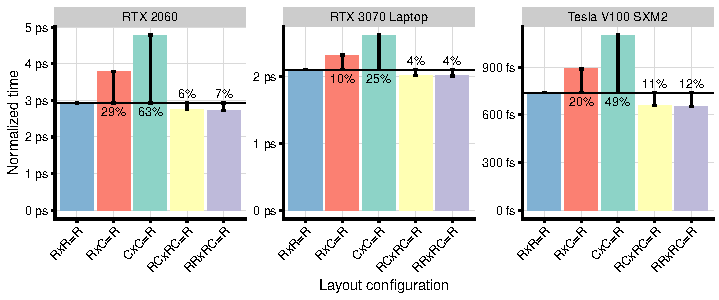
\includegraphics{noarr/plots/matmul_selected.pdf}
    \caption{Speedups of selected layout combinations relative to (row-major) baseline}
    \label{fig:matmul_speedup}
\end{figure}

The result verified that \textbf{RC} is superior to the baseline row-major layout in both input positions. Furthermore, the $R\times C=R$ configuration (often praised on sequential architectures) exhibits worse than the baseline on massively parallel hardware. While this was expected, the primary outcome of this benchmark is methodological: A selection of input and output layouts can be tested systematically without reimplementation effort, while the larger exploration size of the selection (enabled by low coding overhead) provides a solid guarantee that the best-identified solution is indeed a good choice for a high-performance software.


% -----------------------------------------------------------------------------
\subsection{Transformations}\label{sec:transformations}
% -----------------------------------------------------------------------------

The layout-agnostic algorithms can benefit from performance gains achieved by choosing the best layout for a given problem configuration and architecture. However, in real-world scenarios, the layout of the input and output data structures is often prescribed as an inherent part of the algorithm interface or selected by the caller (in the case of generic interfaces).

If the algorithm is complex enough and the performance gap between the prescribed layouts and optimal layouts is high, the data structures may be copied and transformed into their optimally organized counterparts to speed up the algorithm. With \Noarr{}, the transformation can be handled in a generic way. Following our examples with matrices, Listing~\ref{lst:transform} presents the central part of a generic transformer for 2D structures.

\begin{listing}
    \vspace{-10pt}
    \inputmintedcpp{noarr/code-snippets/transform-short.cpp}
    \vspace{-20pt}
    \caption{Key part of transformation routine for 2-index (2D) arrays}
    \label{lst:transform}
\end{listing}

In fact, we are currently extending \Noarr{} to handle the transformations in a generic way for any-dimensional structures, and we are exploring techniques how to select the best way of iterating the structures (e.g., selecting the best ordering of nested loops) in order to optimize memory transfers and caching. However, this research is well beyond the scope of this paper.


\subsubsection{Transformation overhead assessment.}

Employing transformations may be beneficial only under specific circumstances. Simply put, the algorithm must save more execution time than how long it takes to transform all the necessary data. We want to demonstrate the overhead assessment on the previously introduced matrix multiplication example.

We have analyzed the layout transformation overhead for various matrix sizes and layouts. The key results are summarized in Figure~\ref{fig:matmul_comp}. We have observed that in the case of larger matrices ($N>10,000$), the overhead is negligible, primarily because of the asymptotic complexity difference between the transformation algorithm ($\mathcal{O}(N^2)$) and the multiplication ($\mathcal{O}(N^3)$). For smaller matrices (with $N$ around $1000$), the relative ratio of the transformation to computation time expectably increased, and the transformation overhead caused the baseline to perform the best.

\begin{figure}
    \centering
    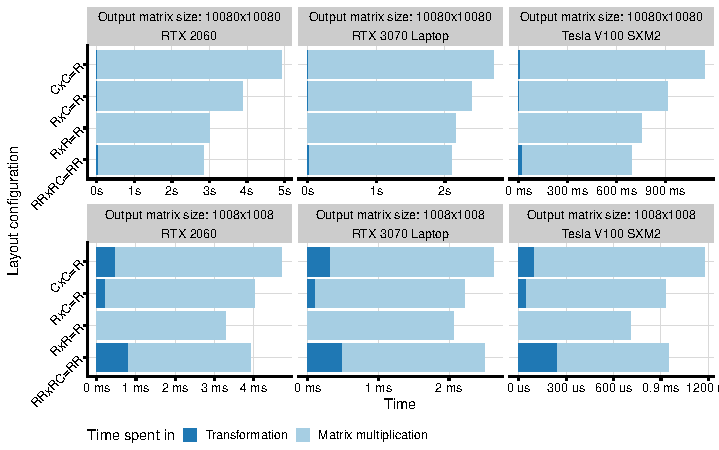
\includegraphics{noarr/plots/matmul_transform.pdf}
    \caption{Layout transformation times compared to actual matrix multiplication times}
    \label{fig:matmul_comp}
\end{figure}

As demonstrated, deciding whether or when a layout transformation can be beneficial may be complicated; however, with \Noarr{}, both the experiments and the actual decision to apply or not to the transformation can be implemented very quickly.

% Finally, it is worth mentioning that the overhead of the transform algorithm can be reduced by selecting an appropriate copy-ordering for different layouts. The example in Listing~\ref{lst:transform} is designed as optimal for row-major layout, but it may not be optimal for other types of transforms. One of the objectives for the future research is to extract meta-information from the layout structures that would allow us to automatically select the optimal transform strategy (e.g., ordering of the nested for-loops).
